\documentclass[conference]{IEEEtran}

% Language setting
% Replace `english' with e.g. `spanish' to change the document language
\usepackage[spanish]{babel}

% Useful packages
\usepackage{amsmath}
\usepackage{graphicx}
\usepackage{url}

% Title and author info
\title{Dashboard Apple Prototype}
\author{\IEEEauthorblockN{Juan David Cotacio Sánchez}}

\begin{document}
\maketitle

\begin{abstract}

\end{abstract}

\section{Introducción}
En el mundo de la tecnología, Apple se destaca como un líder indiscutible, y con nuestro proyecto de Dashboard de Ventas de Apple, hemos combinado la potencia de Python, Django, Pandas, Bootstrap y Plotly para ofrecer una visión integral y dinámica del rendimiento de ventas de esta icónica marca.


\subsection{Como empezar el prototipo}

Para la creación de este prototipo empece en la instalación de Python, DJango, Plotly y Pandas en sistema operativo windows para crear el entorno virtual en el cual iba trabajar mis DashBoard de ventas, además de la creación de mi servidor local con Django donde podemos leer la documentación para crear un Admin para que nuestra información en nuestra DB no sea de facil acceso.
\begin{figure}[h] % Aquí comienza la inclusión de la imagen
    \centering
    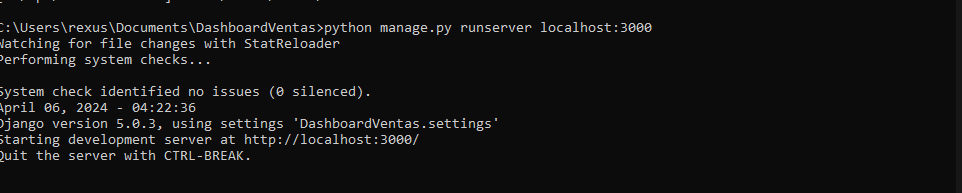
\includegraphics[width=0.5\textwidth]{images/StartUP.png} % Reemplaza 'ruta/de/la/imagen' por la ruta de tu imagen
    \caption{StarUp del Local Server}
    \label{fig:mi_imagen}
\end{figure}

\begin{figure}[h] % Aquí comienza la inclusión de la imagen
    \centering
    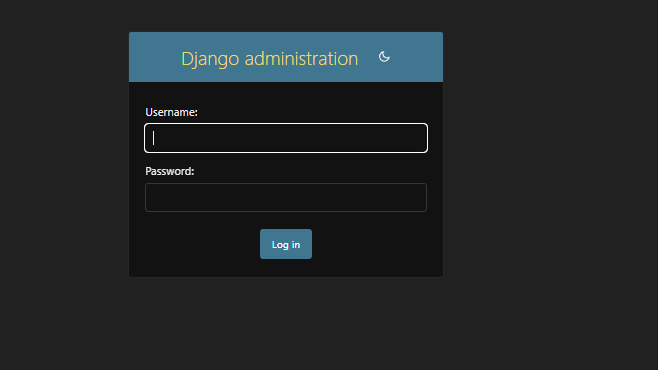
\includegraphics[width=0.5\textwidth]{images/admin.png} % Reemplaza 'ruta/de/la/imagen' por la ruta de tu imagen
    \caption{Admin Django}
    \label{fig:mi_imagen}
\end{figure}

\subsection{Gestion de Grupos y Usuarios}
Depues del acceso ami gestor de datos necesite crear un grupo con cierto privilegios pues se necesita que la información solo sea administrada por lo encargador de las ventas para despues crear usuarios que hagan parte de estos grupos y hagan la gestion de datos.

\begin{figure}[h] % Aquí comienza la inclusión de la imagen
    \centering
    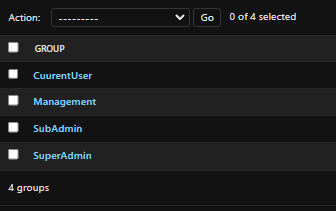
\includegraphics[width=0.4\textwidth]{images/Grupo.png} % Reemplaza 'ruta/de/la/imagen' por la ruta de tu imagen
    \caption{Grupo Django }
    \label{fig:mi_imagen}
\end{figure}

\begin{figure}[h] % Aquí comienza la inclusión de la imagen
    \centering
    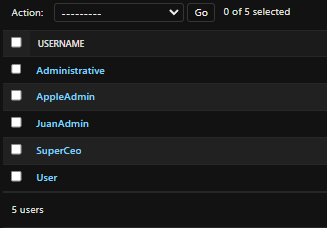
\includegraphics[width=0.4\textwidth]{images/Users.png} % Reemplaza 'ruta/de/la/imagen' por la ruta de tu imagen
    \caption{Usuarios Django }
    \label{fig:mi_imagen}
\end{figure}
\subsection{Creación de nuestra DB}
Para nuestra creación de las ventas realizadas necesitamos empezar a jugar con nuestra base creada al momento de instalar Django, en este caso necesitamos irno al models.py para poner nuestros tipos de datos y la cantidad de estos mismos decici crear dos tipos de ventas, uno que sean sus ventas mensuales por continentes y otros por porductos con sus respectivos tipos de datos.

Tambien en la consola realice la debida migración de mis datos a mi db en este caso realize 3 migraciones pues realice ciertos respectivos cambios para esto es necesario cuando cambiamos cosas de nuestro modelo.

Para la organizacion de nuestros datos en Django lo que hice fue jugar con nuestro admin.py, en la documentación nos brindan una un array listDisplay para poder mostrar de mejor manera nuestros datos.



\begin{figure}[h] % Aquí comienza la inclusión de la imagen
    \centering
    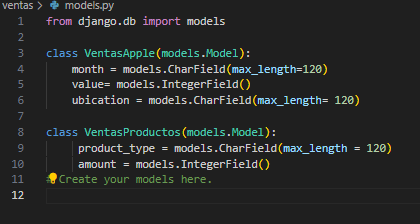
\includegraphics[width=0.4\textwidth]{images/Models.png} % Reemplaza 'ruta/de/la/imagen' por la ruta de tu imagen
    \caption{Modelo Python}
    \label{fig:mi_imagen}
\end{figure}

\begin{figure}[h] % Aquí comienza la inclusión de la imagen
    \centering
    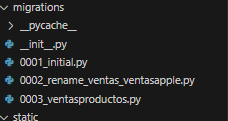
\includegraphics[width=0.4\textwidth]{images/Migrations.png} % Reemplaza 'ruta/de/la/imagen' por la ruta de tu imagen
    \caption{Migraciones}
    \label{fig:mi_imagen}
\end{figure}
\begin{figure}[h] % Aquí comienza la inclusión de la imagen
    \centering
    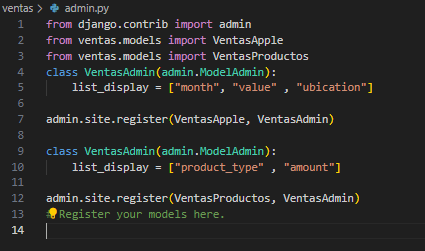
\includegraphics[width=0.4\textwidth]{images/adminpy.png} % Reemplaza 'ruta/de/la/imagen' por la ruta de tu imagen
    \caption{Admin Python}
    \label{fig:mi_imagen}
\end{figure}

\begin{figure}[h] % Aquí comienza la inclusión de la imagen
    \centering
    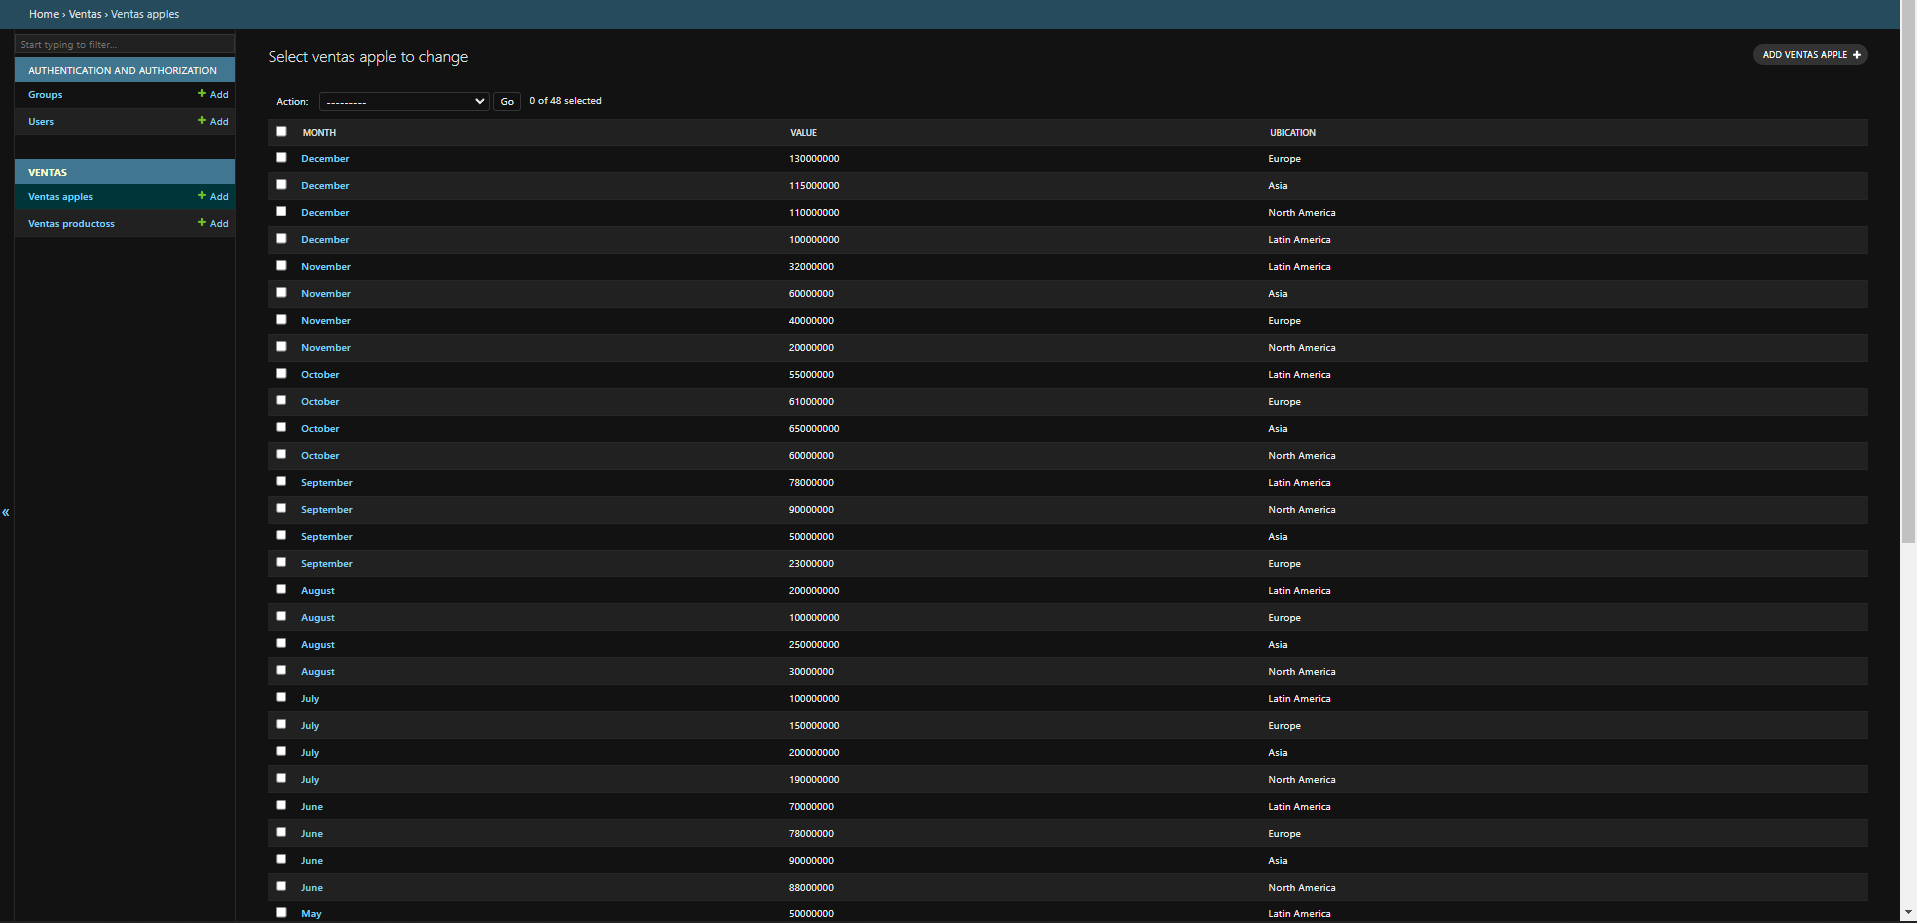
\includegraphics[width=0.4\textwidth]{images/Sells.png} % Reemplaza 'ruta/de/la/imagen' por la ruta de tu imagen
    \caption{Datos de la ventas Mensuales }
    \label{fig:mi_imagen}
\end{figure}
\begin{figure}[h] % Aquí comienza la inclusión de la imagen
    \centering
    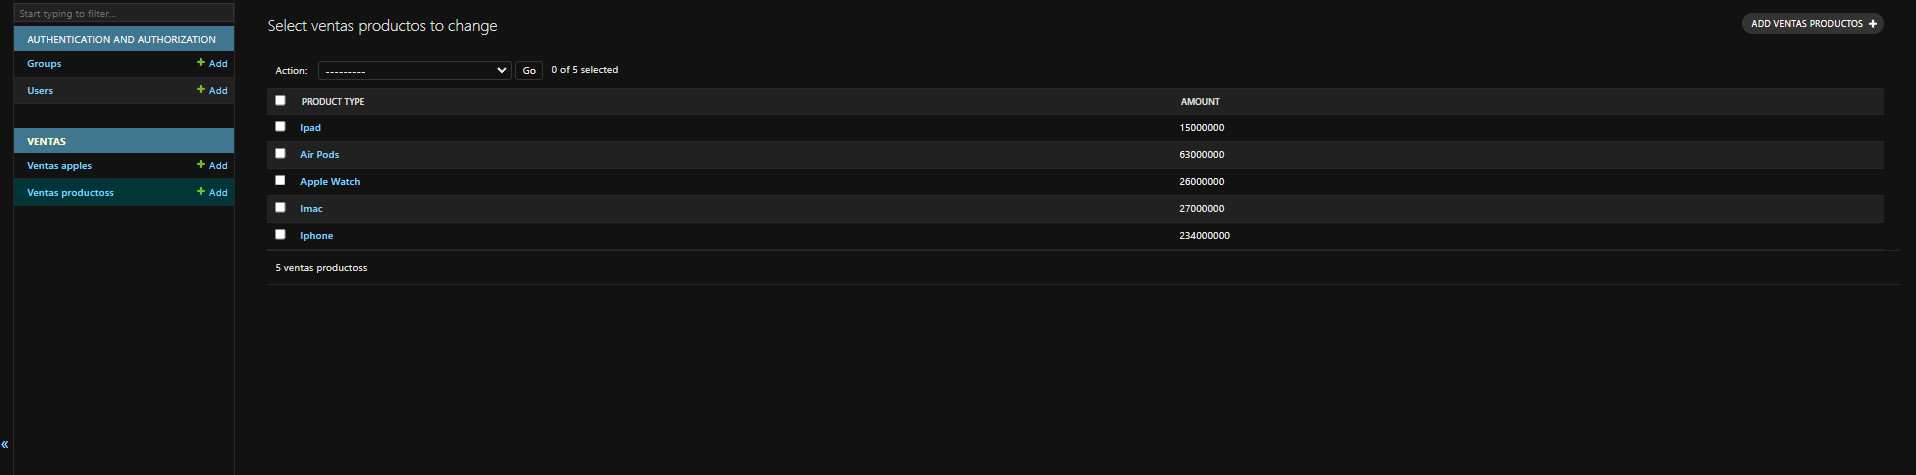
\includegraphics[width=0.4\textwidth]{images/Ventas.png} % Reemplaza 'ruta/de/la/imagen' por la ruta de tu imagen
    \caption{Datos de ventas por productos}
    \label{fig:mi_imagen}
\end{figure}



\subsection{Implementación del Views}

La views fue una de las partes mas complejas en ese proyecto pues es donde basicamente vamos a mostrar los datos de nuestra DB de manera dinamica, en este punto es donde usamos Plotlys para nuestra graficas, para tener una mejor visión de nuestros datos y dashboards complementandose con Pandas.
Basicamente en este punto necesitaremos realizar varias intancias de nuestros datos en la base datos para así traerlos todos y empezar la gestion, para poder empezar a interactuar nuestros datos y las graficas de Plotly necesitaremos usar DataFrames con los datos que necesitaremos, en este hubieron graficas que yo solo queria traer algunos datos entonces se pasaba esos parametros, ademas usaremos HTML y CSS para poder mostrar en una pagina web, por lo que necesitaremos retornar esta información a nuestro HTML.

\begin{figure}[h] % Aquí comienza la inclusión de la imagen
    \centering
    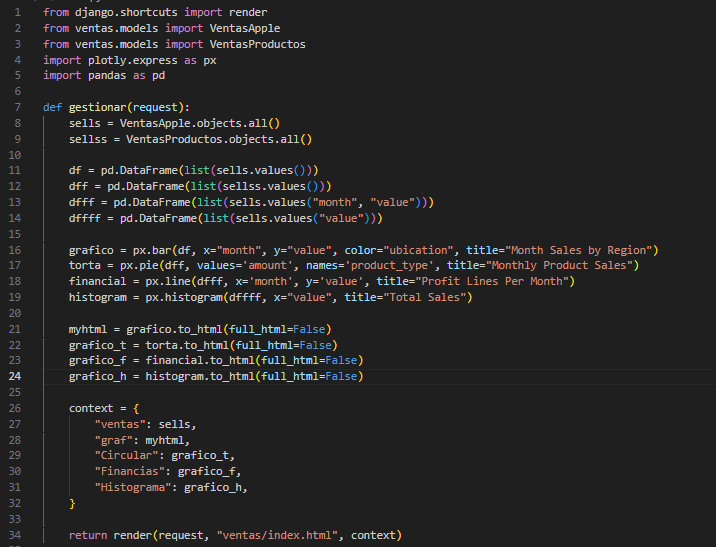
\includegraphics[width=0.4\textwidth]{images/views.png} % Reemplaza 'ruta/de/la/imagen' por la ruta de tu imagen
    \caption{Implementació Views}
    \label{fig:mi_imagen}
\end{figure}


\subsection{Integración de nuestro HTML Y CSS}
Para poder mostrar un DashBoard con nuestra DB necesitaremos crear nuestro templates en una carpeta Statica para poder importarlo en nuestro HTML, hacemos la estructura basica de nuestro HTML, importamos boostrap para poder darle un mejor diseño, una de la cosas investigativas fue la manera en como importaba mis sources y css al html, para eso usaremos nuestra carpeta statica y la cargaremos al incicio y es seguir la estructura que seguirimos por defecto.Z
\begin{figure}[h] % Aquí comienza la inclusión de la imagen
    \centering
    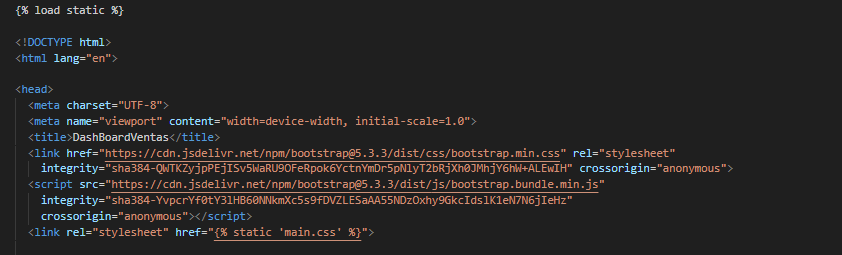
\includegraphics[width=0.5\textwidth]{images/Static .png} % Reemplaza 'ruta/de/la/imagen' por la ruta de tu imagen
    \caption{Llamado Carpeta Static}
    \label{fig:mi_imagen}
\end{figure}

\begin{figure}[h] % Aquí comienza la inclusión de la imagen
    \centering
    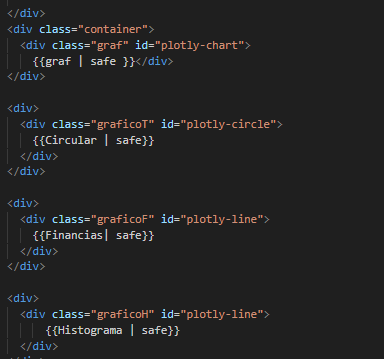
\includegraphics[width=0.5\textwidth]{images/Llamado Views.png} % Reemplaza 'ruta/de/la/imagen' por la ruta de tu imagen
    \caption{Manera de traer nuestros datos de views al HTML}
    \label{fig:mi_imagen}
\end{figure}

\subsection{Vista General del Prototipo}
En la vista general de mi protipo se logro la gestion de nuestros datos por Django y además de eso usar nuestras herramientas clasicas con nuevos frameworks y librerias, como lo son Plotly y Pandas, cargar los datos de manera dinamica.

\begin{figure}[h] % Aquí comienza la inclusión de la imagen
    \centering
    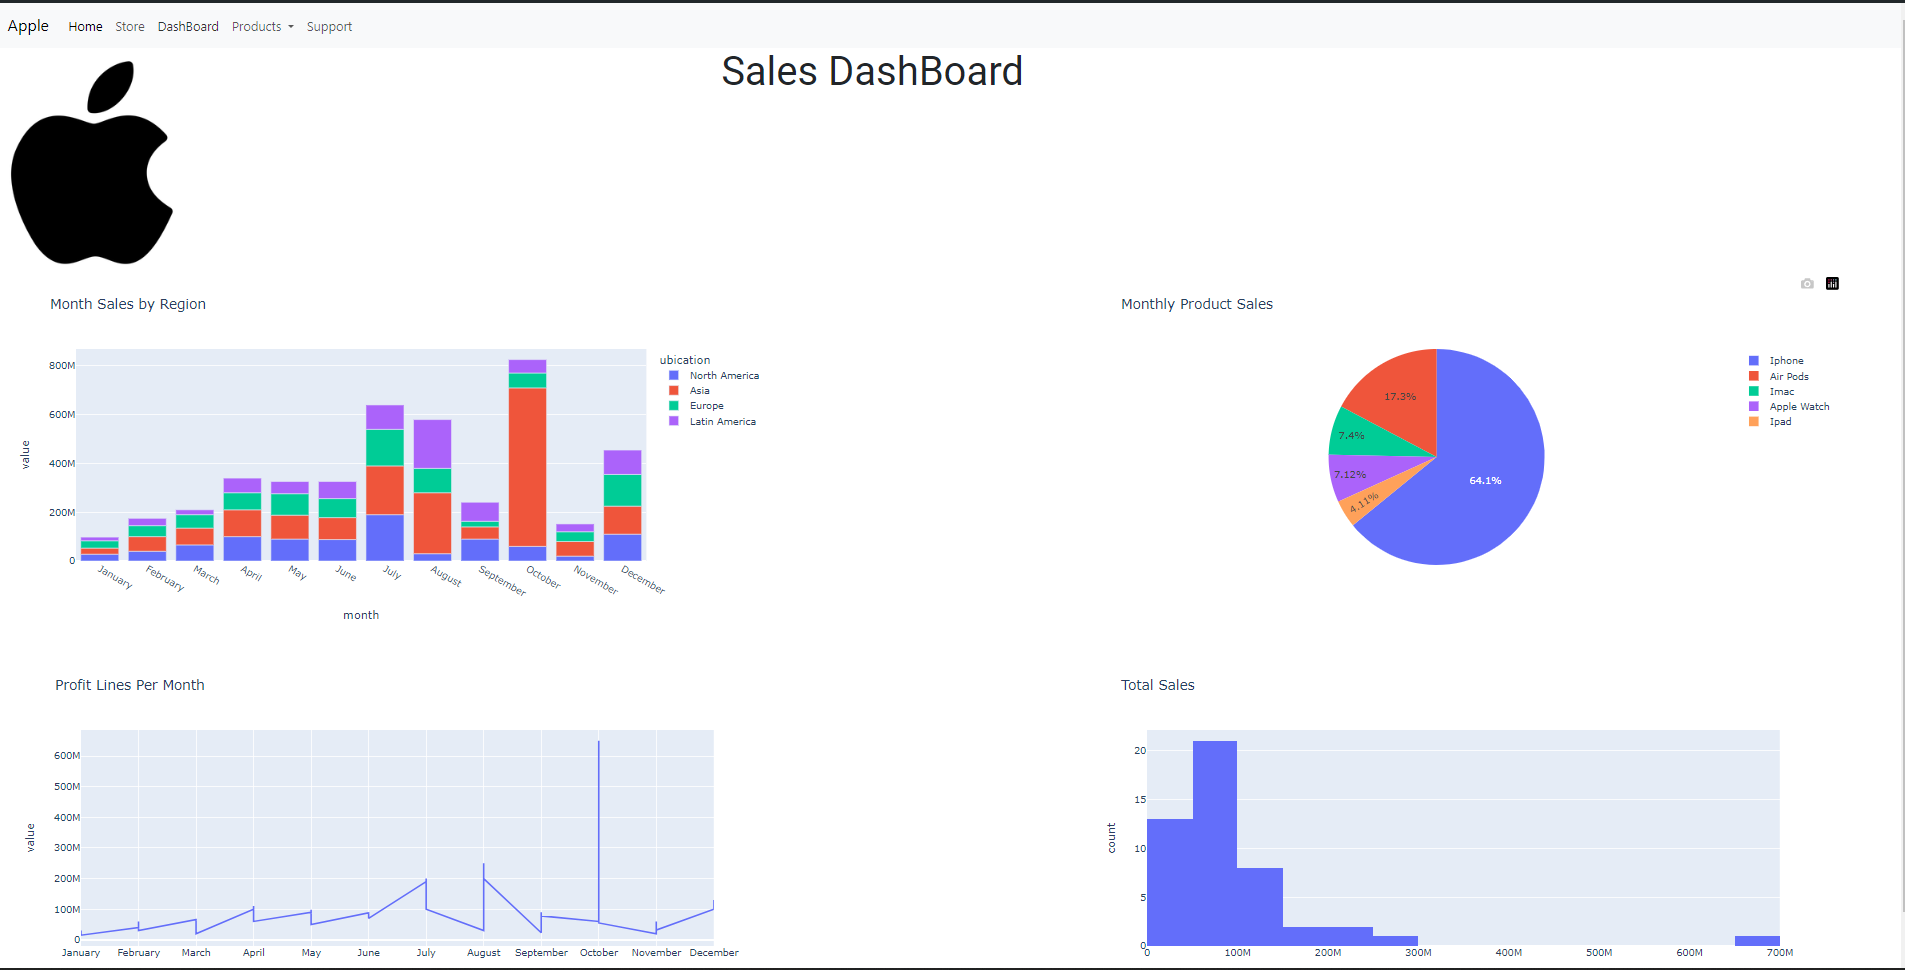
\includegraphics[width=0.5\textwidth]{images/DashBoardViews.png} % Reemplaza 'ruta/de/la/imagen' por la ruta de tu imagen
    \caption{Vista Final Del Prototipo}
    \label{fig:mi_imagen}
\end{figure}

\subsection{Instructivo}
Para que el juego se pueda disfrutar en terminos general se debe ajustar siempre valores, para que el contenido se adapte a la pantalla y no se vea desproporcioando se pueda utilizar la combinacion de teclas "ctrl + +" o en su defecto "ctrl + -", estos valores son adaptables al gusto del usuario pero para resoluciones 1920 x 1080, el 80 porciento queda perfectamente ancajado.

Este dashboard maneja un navBar para tener un diseño similar al de Apple es interactivo pero para mas comodidad del usuario iniciar el servidor en el puerto 3000 para no tener ningun incoveniente.
\begin{figure}[h] % Aquí comienza la inclusión de la imagen
    \centering
    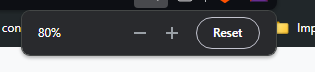
\includegraphics[width=0.5\textwidth]{images/80.png} % Reemplaza 'ruta/de/la/imagen' por la ruta de tu imagen
    \caption{Zoom para resoluciones 1920 x 1080}
    \label{fig:mi_imagen}
\end{figure}


\end{document}

